\documentclass[11pt, a4paper]{article}

\usepackage[margin=2.5cm]{geometry}
\usepackage{amsmath, amssymb, amsthm}
\usepackage{bm}
\usepackage{xcolor}
\usepackage{booktabs}
\usepackage{array}
\usepackage{tikz}
\usetikzlibrary{arrows.meta, positioning, shapes.geometric,
                fit, backgrounds, calc}
\usepackage{algorithm}
\usepackage{algpseudocode}
\usepackage{hyperref}
\usepackage{enumitem}
\usepackage{mdframed}
\usepackage{caption}

% ── Colours ────────────────────────────────────────────────────────────────
\definecolor{aifblue}{RGB}{30,90,180}
\definecolor{aifgreen}{RGB}{0,140,80}
\definecolor{aifgray}{RGB}{90,90,90}
\definecolor{aifred}{RGB}{180,40,40}
\definecolor{aifpurple}{RGB}{120,40,160}
\definecolor{aiforange}{RGB}{200,110,0}
\definecolor{boxbg}{RGB}{240,246,255}
\definecolor{warningbg}{RGB}{255,248,230}
\definecolor{greenbg}{RGB}{235,250,238}
\definecolor{purplebg}{RGB}{248,240,255}

\newmdenv[backgroundcolor=boxbg,linecolor=aifblue,
  linewidth=1.5pt,roundcorner=4pt,
  innertopmargin=8pt,innerbottommargin=8pt]{keybox}
\newmdenv[backgroundcolor=warningbg,linecolor=aiforange,
  linewidth=1.5pt,roundcorner=4pt,
  innertopmargin=8pt,innerbottommargin=8pt]{notebox}
\newmdenv[backgroundcolor=greenbg,linecolor=aifgreen,
  linewidth=1.5pt,roundcorner=4pt,
  innertopmargin=8pt,innerbottommargin=8pt]{resultbox}
\newmdenv[backgroundcolor=purplebg,linecolor=aifpurple,
  linewidth=1.5pt,roundcorner=4pt,
  innertopmargin=8pt,innerbottommargin=8pt]{pymdpbox}

% ── Macros ──────────────────────────────────────────────────────────────────
\newcommand{\vect}[1]{\bm{#1}}
\newcommand{\mat}[1]{\mathbf{#1}}
\newcommand{\FE}{\mathcal{F}}
\newcommand{\EFE}{\mathcal{G}}
\newcommand{\norm}[1]{\left\|#1\right\|}
\newcommand{\Pip}{\mat{\Pi}_p}
\newcommand{\Pisl}{\mat{\Pi}_s^{\mathrm{low}}}
\newcommand{\Pish}{\Pi_s^{\mathrm{high}}}
\newcommand{\epsp}{\vect{\varepsilon}_p}
\newcommand{\epss}{\vect{\varepsilon}_s}
\newcommand{\KL}{D_{\mathrm{KL}}}

\title{%
  \textbf{\Large Hierarchical Active Inference with \texttt{pymdp}}\\[4pt]
  \large Discrete High-Level Agent (Policy Selection via $\EFE$)\\
  $+$ Continuous Low-Level Agent (Trajectory Tracking)
}
\author{}
\date{}

\begin{document}
\maketitle\thispagestyle{empty}
\tableofcontents\newpage

% ═══════════════════════════════════════════════════════════════════════════
\section{Overview and Motivation}

The previous version of the hierarchical model used a hand-rolled discrete
belief update with passive perception only. This document describes the
corrected formulation, implemented using the \texttt{inferactively-pymdp}
library (v0.0.7), which provides:

\begin{itemize}[noitemsep]
  \item Marginal message passing for state inference (replacing softmax heuristic)
  \item Expected free energy $\EFE$ for \emph{active} policy selection
  \item A clean separation of epistemic and pragmatic value in $\EFE$
  \item Three candidate vertex-potential proxies, testable against EEG data
\end{itemize}

\begin{keybox}
\textbf{Key upgrade from passive to active inference.}
The previous agent detected surprise but never \emph{decided} anything.
The \texttt{pymdp} agent selects between two policies at every timestep:
\[
  \pi \in \{\underbrace{\textsc{Track}}_{0},\;
            \underbrace{\textsc{Interrupt}}_{1}\}
\]
Policy selection is driven by expected free energy $\EFE(\pi)$, which
balances epistemic value (resolving uncertainty about the stimulus) against
pragmatic cost (disrupting the ongoing trajectory). This provides a principled
threshold: weak stimuli do not cross the $\EFE$ decision boundary and
produce \emph{zero} kinematic perturbation; strong stimuli do.
\end{keybox}

% ═══════════════════════════════════════════════════════════════════════════
\section{Generative Model Matrices}

\subsection{Likelihood matrix $\mat{A}$}
\begin{equation}
  \mat{A} \in [0,1]^{N_o \times N_s},
  \qquad
  A_{o,s} = p(o_t = o \mid s_t = s),
\end{equation}
with $N_o = 2$ (no-stim / stim) and $N_s = 3$ (TRACK / SURP / RECOVER):
\begin{equation}
  \mat{A} =
  \begin{pmatrix}
    0.95 & 0.05 & 0.90 \\
    0.05 & 0.95 & 0.10
  \end{pmatrix}.
\end{equation}
SURP is the only state that strongly predicts stimulus presence.

\subsection{Transition tensor $\mat{B}(\bar{e})$}
\begin{equation}
  \mat{B} \in [0,1]^{N_s \times N_s \times N_\pi},
  \qquad
  B_{s',s,\pi} = p(s_t = s' \mid s_{t-1} = s,\; \pi_t = \pi).
\end{equation}
Columns sum to 1. The tensor has two slices, one per policy.
Both slices are modulated by normalised efference copy
$\bar{e}(t) = \norm{\vect{a}(t)}/a_{\max} \in [0,1]$:
\begin{align}
  p(\textsc{Track} \to \textsc{Surp} \mid \pi)
    &= p_0^\pi + \alpha_B\,\bar{e}, \\
  p(\textsc{Surp}  \to \textsc{Rec}  \mid \pi)
    &= q_0^\pi + \alpha_B\,\bar{e}, \\
  p(\textsc{Rec}   \to \textsc{Track}\mid \pi)
    &= r_0^\pi + \alpha_B\,\bar{e}.
\end{align}
The \textsc{Interrupt} policy has higher base rates $q_0^1 \gg q_0^0$,
$r_0^1 \gg r_0^0$: it resolves surprise faster.

\begin{notebox}
\textbf{Dynamic B in \texttt{pymdp}.}
\texttt{pymdp} does not natively support step-varying $\mat{B}$.
We recompute $\mat{B}(\bar{e}(t))$ at every timestep and assign it
directly to \texttt{agent.B} before calling
\texttt{agent.infer\_policies()}. No agent reinitialisation is required.
\end{notebox}

\subsection{Preference vector $\mat{C}$}
Log-preferences over observations encode that the agent prefers not to
observe surprising stimuli:
\begin{equation}
  \mat{C} = \bigl[\ln 0.9,\; \ln 0.1\bigr]^\top.
\end{equation}
This enters the \emph{pragmatic} term of $\EFE$ (Sec.~\ref{sec:efe}).

\subsection{Prior over initial states $\mat{D}$}
\begin{equation}
  \mat{D} = [0.95,\; 0.025,\; 0.025]^\top.
\end{equation}

% ═══════════════════════════════════════════════════════════════════════════
\section{State Inference — Marginal Message Passing}

At each timestep \texttt{pymdp} computes the posterior
$q(s_t) \in \Delta^{N_s}$ via marginal message passing:

\paragraph{Step 1 — Prior prediction.}
\begin{equation}
  \vect{s}_{\mathrm{prior}} = \mat{B}_{:,:,\hat{\pi}}\;\vect{q}(s_{t-1}),
\end{equation}
where $\hat{\pi}$ is the policy selected at the previous step.

\paragraph{Step 2 — Likelihood update.}
\begin{equation}
  \ln q(s_t) = \ln \vect{s}_{\mathrm{prior}}
             + \mat{A}_{o_t,:}^\top
  \quad\Rightarrow\quad
  q(s_t) = \sigma\!\left(\ln\vect{s}_{\mathrm{prior}}
                       + \ln\mat{A}_{o_t,:}\right),
\end{equation}
where $\sigma(\cdot)$ is the softmax.

\paragraph{Surprise.}
\begin{equation}
  p(o_t) = \mat{A}_{o_t,:}\;\vect{q}(s_t),
  \qquad
  \xi_t = -\ln p(o_t).
  \label{eq:surprise}
\end{equation}

\begin{pymdpbox}
\textbf{\texttt{pymdp} call:}
\texttt{qs = agent.infer\_states(obs)}\\
Returns \texttt{qs[0]}, shape \texttt{(NUM\_STATES,)}.
\texttt{obs} is a list of integers, one per modality.
\end{pymdpbox}

% ═══════════════════════════════════════════════════════════════════════════
\section{Policy Selection — Expected Free Energy}
\label{sec:efe}

\subsection{Definition of $\EFE$}
The expected free energy for policy $\pi$ over a horizon $\tau$ is:
\begin{equation}
  \EFE(\pi) = \sum_{\tau} \mathbb{E}_{q(o_\tau,s_\tau|\pi)}
  \Bigl[\underbrace{\ln q(s_\tau|\pi) - \ln q(s_\tau|o_\tau,\pi)}_{\text{epistemic value}}
  \;+\; \underbrace{\ln q(o_\tau|\pi) - \ln p(o_\tau)}_{\text{pragmatic value}}\Bigr].
  \label{eq:efe_full}
\end{equation}

For one-step lookahead ($\tau=1$) this reduces to:
\begin{equation}
  \EFE(\pi)
  = \underbrace{-\mathbb{E}_{q(s|\pi)}\bigl[H[\mat{A}_{:,s}]\bigr]}_{\text{epistemic: info gain}}
  \;-\; \underbrace{\mathbb{E}_{q(o|\pi)}\bigl[\ln p(o)\bigr]}_{\text{pragmatic: preferences}},
  \label{eq:efe_decomp}
\end{equation}
where $H[\mat{A}_{:,s}] = -\sum_o A_{o,s}\ln A_{o,s}$ is the entropy of
the likelihood column for state $s$, and $\ln p(o) = \mat{C}$.

\begin{keybox}
\textbf{Interpretation for the two-policy model.}
\begin{itemize}[noitemsep]
  \item \textbf{Epistemic term:} \textsc{Interrupt} has lower expected
        likelihood entropy because it routes the agent through RECOVER
        (a more predictable state) — it \emph{resolves} uncertainty.
  \item \textbf{Pragmatic term:} \textsc{Interrupt} incurs a pragmatic
        cost because entering SURP risks observing the unpreferred stimulus.
        But this is offset by the epistemic gain.
  \item \textbf{Threshold:}
        $\EFE(\textsc{Interrupt}) < \EFE(\textsc{Track})$ only when
        surprise $\xi_t$ is large enough — this is the free threshold
        mechanism that produces all-or-nothing perturbations.
\end{itemize}
\end{keybox}

\subsection{Policy posterior}
\begin{equation}
  q(\pi) = \sigma\!\left(-\gamma_G\,\EFE(\pi)\right),
  \qquad
  q(\pi) \in \Delta^{N_\pi},
  \label{eq:q_pi}
\end{equation}
where $\gamma_G > 0$ is the policy precision (temperature).
High $\gamma_G$ makes policy selection more deterministic.

\begin{pymdpbox}
\textbf{\texttt{pymdp} calls:}\\
\texttt{q\_pi, G = agent.infer\_policies()}\\
Returns \texttt{q\_pi} shape \texttt{(NUM\_POLICIES,)} and
\texttt{G} shape \texttt{(NUM\_POLICIES,)}.\\[4pt]
\texttt{action = agent.sample\_action()}\\
Returns action index (0 or 1) drawn from \texttt{q\_pi}.
\end{pymdpbox}

% ═══════════════════════════════════════════════════════════════════════════
\section{Precision Coupling}

\subsection{Surprise pulse $\gamma(t)$ — gated by policy}
The critical upgrade from the previous version: $\gamma$ only accumulates
when the \textsc{Interrupt} policy is selected.
\begin{equation}
  \dot{\gamma} = -\frac{\gamma}{\tau_\gamma}
    + \lambda_\gamma\;\xi_t\;\underbrace{\mathbb{1}[\pi_t = \textsc{Interrupt}]}_{\text{policy gate}},
  \qquad \gamma \geq 0.
  \label{eq:gamma_gated}
\end{equation}
This makes the kinematic perturbation \emph{conditional on policy selection}:
stimuli that do not cross the $\EFE$ threshold produce zero kinematic
effect regardless of their physical intensity.

\subsection{Low-level sensory precision}
\begin{equation}
  \Pisl(t) = \frac{1}{1+\gamma(t)}\;\mat{\Pi}_s^{\mathrm{base}},
  \label{eq:pisl}
\end{equation}
z-entries always zero (unobserved axis).

\subsection{High-level sensory precision}
\begin{equation}
  \Pish(t) = \frac{\Pi_s^{\mathrm{high,base}}\,(1+\gamma(t))}
                  {1 + \alpha_{\mathrm{eff}}\,\bar{e}(t)}.
  \label{eq:pish}
\end{equation}
Independent of $\Pisl$ — no conservation law.

% ═══════════════════════════════════════════════════════════════════════════
\section{Low-Level Continuous Agent}

Unchanged from the single-agent formulation except $\Pisl(t)$ is now
time-varying via Eq.~(\ref{eq:pisl}).

\subsection{Belief update}
\begin{equation}
  \dot{\vect{\mu}} = \vect{f}_{\mathrm{model}}(\vect{\mu}, \vect{a})
    + \kappa_\mu\bigl(\Pisl(t)\,\epss - \Pip\,\epsp\bigr).
\end{equation}

\subsection{Precision-modulated PD action}
\begin{align}
  u_1 &= \frac{m_1}{1+\gamma}\bigl[K_P(p_1^* - \mu_{p_1})
         + K_D(v_1^* - \mu_{v_1})\bigr], \\
  u_2 &= \frac{m_2}{1+\gamma}\bigl[K_P(p_2^* - \mu_{p_2})
         + K_D(v_2^* - \mu_{v_2})\bigr] + m_2 g.
\end{align}

% ═══════════════════════════════════════════════════════════════════════════
\section{Vertex Potential Proxies}
\label{sec:vp}

Three candidates are stored, all testable against empirical EEG amplitudes:

\begin{center}
\renewcommand{\arraystretch}{1.5}
\begin{tabular}{llp{5.5cm}}
\toprule
\textbf{Symbol} & \textbf{Expression} & \textbf{Neural interpretation} \\
\midrule
$\mathrm{VP}_{\Pi\varepsilon}$ &
  $\Pish(t)\cdot\norm{\vect{\varepsilon}_{s,xy}}$ &
  Precision-weighted prediction error;
  attenuated by efference via $\Pish$ denominator \\
$\mathrm{VP}_{\EFE}$ &
  $-\min_\pi \EFE(\pi)$ &
  Negative minimum EFE; peaks when one policy is strongly preferred \\
$\mathrm{VP}_{q\pi}$ &
  $q(\pi=\textsc{Interrupt})$ &
  Posterior probability of interruption;
  simplest proxy, directly interpretable \\
\bottomrule
\end{tabular}
\end{center}

\paragraph{Predicted anti-correlation.}
$\bar{e}(t)$ large (movement) suppresses $\Pish$ via its denominator
$\Rightarrow$ $\mathrm{VP}_{\Pi\varepsilon}$ smaller. Simultaneously,
$\bar{e}$ increases $p(\textsc{Track}\to\textsc{Surp})$ via $\mat{B}$,
so a stimulus that crosses the $\EFE$ threshold does so with larger $\xi$
and drives a larger $\gamma$ pulse $\Rightarrow$ bigger kinematic disruption.
The two effects are independent, share one cause ($\bar{e}$), and produce
opposite signs in the two observables.

% ═══════════════════════════════════════════════════════════════════════════
\section{Full Algorithm}

\begin{algorithm}[H]
\caption{Hierarchical AIF — \texttt{pymdp} High-Level Agent}
\label{alg:pymdp}
\begin{algorithmic}[1]
\Require Parameters; noise arrays; \texttt{pymdp} Agent initialised with
         $\mat{A}, \mat{B}_0, \mat{C}, \mat{D}$
\State \textbf{Init:} $\vect{x}_{\mathrm{real}}, \vect{\mu} \leftarrow \vect{x}_0$;\;
       $\gamma \leftarrow 0$;\;
       $\vect{a}_{\mathrm{prev}} \leftarrow \vect{0}$;\;
       $\pi \leftarrow \textsc{Track}$
\For{$k = 0,\ldots,N-1$}
  \State $t \leftarrow k\Delta t$;\quad
         $\vect{x}^* \leftarrow$ \Call{DesiredState}{$t$};\quad
         $o_t \leftarrow \mathbb{1}[\text{stimulus}]$
  \State
  \State \textbf{--- Efference copy ---}
  \State $\bar{e} \leftarrow \norm{\vect{a}_{\mathrm{prev}}}/a_{\max}$
  \State
  \State \textbf{--- High-level: update B ---}
  \State \texttt{agent.B} $\leftarrow \mat{B}(\bar{e})$
         \hfill{\color{aifpurple}\textit{pymdp: direct assignment}}
  \State
  \State \textbf{--- High-level: state inference ---}
  \State \texttt{qs} $\leftarrow$ \texttt{agent.infer\_states([}$o_t$\texttt{])}
         \hfill{\color{aifpurple}\textit{pymdp: marginal message passing}}
  \State $q(s_t) \leftarrow$ \texttt{qs[0]};\quad
         $\xi \leftarrow -\ln(\mat{A}_{o_t,:}\,q(s_t))$
  \State
  \State \textbf{--- High-level: policy selection ---}
  \State \texttt{q\_pi, G} $\leftarrow$ \texttt{agent.infer\_policies()}
         \hfill{\color{aifpurple}\textit{pymdp: expected free energy}}
  \State $\pi \leftarrow$ \texttt{agent.sample\_action()[0]}
         \hfill{\color{aifpurple}\textit{pymdp: softmax draw}}
  \State
  \State \textbf{--- Precision pulse (policy-gated) ---}
  \State $\gamma \leftarrow \gamma
         + \bigl(-\gamma/\tau_\gamma
         + \lambda_\gamma\,\xi\,\mathbb{1}[\pi{=}\textsc{Interrupt}]\bigr)\Delta t$
  \State
  \State \textbf{--- Low-level precision ---}
  \State $\sigma \leftarrow 1/(1+\gamma)$;\quad
         $\Pisl \leftarrow \sigma\,\mat{\Pi}_s^{\mathrm{base}}$;\quad
         $\Pish \leftarrow \Pi_s^{\mathrm{h,base}}(1+\gamma)/(1+\alpha_{\mathrm{eff}}\bar{e})$
  \State
  \State \textbf{--- Low-level: observe, errors, free energy ---}
  \State $\vect{y}_{\mathrm{obs}} \leftarrow$ observe $x$-$y$ only
  \State $\epsp \leftarrow \vect{\mu} - \vect{x}^*$;\quad
         $\epss \leftarrow \vect{y}_{\mathrm{obs}} - \vect{\mu}$
  \State $\FE_{\mathrm{low}} \leftarrow
         \tfrac{1}{2}(\epsp^\top\Pip\epsp + \epss^\top\Pisl\epss)$
  \State
  \State \textbf{--- Low-level: action ---}
  \State $u_1 \leftarrow \sigma\,m_1[K_P(\ldots) + K_D(\ldots)]$;\quad
         $u_2 \leftarrow \sigma\,m_2[\ldots] + m_2 g$;\quad
         clip;\quad $\vect{a}_{\mathrm{prev}} \leftarrow \vect{a}$
  \State
  \State \textbf{--- World + belief update ---}
  \State $\vect{x}_{\mathrm{real}} \leftarrow \vect{x}_{\mathrm{real}}
         + \vect{f}_{\mathrm{proc}}(\ldots)\Delta t$;\quad
         $\vect{\mu} \leftarrow \vect{\mu}
         + [\vect{f}_{\mathrm{model}} + \kappa_\mu(\Pisl\epss
         - \Pip\epsp)]\Delta t$
  \State
  \State \textbf{--- Store VP proxies ---}
  \State $\mathrm{VP}_{\Pi\varepsilon} \leftarrow \Pish\norm{\vect{\varepsilon}_{s,xy}}$;\quad
         $\mathrm{VP}_{\EFE} \leftarrow -\min_\pi G(\pi)$;\quad
         $\mathrm{VP}_{q\pi} \leftarrow q(\pi{=}\textsc{Interrupt})$
\EndFor
\end{algorithmic}
\end{algorithm}

% ═══════════════════════════════════════════════════════════════════════════
\section{System Diagram}

\begin{figure}[ht]
\centering
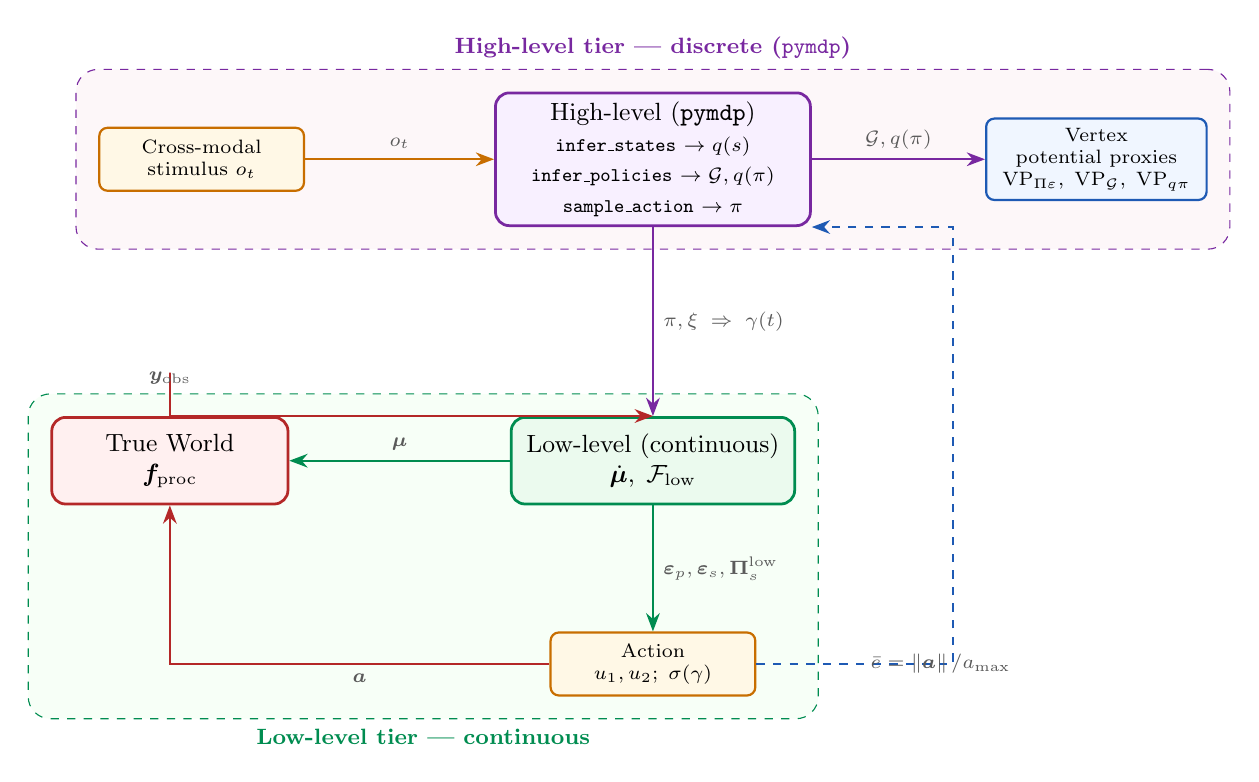
\begin{tikzpicture}[
  node distance=1.6cm and 2.2cm,
  every node/.style={font=\small},
  hibox/.style={draw,rounded corners=5pt,minimum height=1.2cm,
    minimum width=4.0cm,align=center,fill=purplebg,draw=aifpurple,line width=1pt},
  lobox/.style={draw,rounded corners=5pt,minimum height=1.1cm,
    minimum width=3.6cm,align=center,fill=greenbg,draw=aifgreen,line width=1pt},
  wdbox/.style={draw,rounded corners=5pt,minimum height=1.1cm,
    minimum width=3.0cm,align=center,fill=red!6,draw=aifred,line width=1pt},
  smbox/.style={draw,rounded corners=3pt,minimum height=0.8cm,
    minimum width=2.6cm,align=center,font=\scriptsize,
    fill=warningbg,draw=aiforange,line width=0.8pt},
  vpbox/.style={draw,rounded corners=3pt,minimum height=0.9cm,
    minimum width=2.8cm,align=center,font=\scriptsize,
    fill=boxbg,draw=aifblue,line width=0.8pt},
  arr/.style={-Stealth,thick},
  lb/.style={font=\scriptsize\itshape,color=aifgray}
]

\node[hibox] (hl)
  {High-level (\texttt{pymdp})\\
   \scriptsize\texttt{infer\_states} $\to q(s)$\\
   \scriptsize\texttt{infer\_policies} $\to \EFE, q(\pi)$\\
   \scriptsize\texttt{sample\_action} $\to \pi$};

\node[smbox, left=2.4cm of hl]  (stim) {Cross-modal\\stimulus $o_t$};
\node[vpbox, right=2.2cm of hl] (vp)
  {Vertex\\potential proxies\\
   $\mathrm{VP}_{\Pi\varepsilon},\;\mathrm{VP}_{\EFE},\;\mathrm{VP}_{q\pi}$};

\node[lobox, below=2.4cm of hl]   (lo)   {Low-level (continuous)\\$\dot{\vect{\mu}},\;\FE_{\mathrm{low}}$};
\node[wdbox, left=2.8cm of lo]    (world){True World\\$\vect{f}_{\mathrm{proc}}$};
\node[smbox, below=1.6cm of lo]   (act)  {Action\\$u_1,u_2;\;\sigma(\gamma)$};

% Stim → HL
\draw[arr,aiforange]
  (stim.east) -- node[above,lb]{$o_t$} (hl.west);

% HL → VP
\draw[arr,aifpurple]
  (hl.east) -- node[above,lb]{$\EFE,q(\pi)$} (vp.west);

% HL → LO (precision gate)
\draw[arr,aifpurple]
  (hl.south) -- node[right,lb]{$\pi,\xi\;\Rightarrow\;\gamma(t)$} (lo.north);

% LO → World
\draw[arr,aifgreen]
  (lo.west) -- node[above,lb]{$\vect{\mu}$} (world.east);

% World → LO (obs)
\draw[arr,aifred]
  (world.north) -- ++(0,0.55)
  -- node[above,lb]{$\vect{y}_{\mathrm{obs}}$}
  (lo.north -| world.north) -- (lo.north);

% LO → action
\draw[arr,aifgreen]
  (lo.south) -- node[right,lb]{$\epsp,\epss,\Pisl$} (act.north);

% Action → world
\draw[arr,aifred]
  (act.west) -- node[below,lb]{$\vect{a}$}
  (world.south |- act.west) -- (world.south);

% Efference copy: action → HL (dashed blue)
\draw[arr,aifblue,dashed,thick]
  (act.east)
  -- node[right,lb,xshift=2pt]{$\bar{e}=\norm{\vect{a}}/a_{\max}$}
  ++(2.5,0)
  |- (hl.south east);

% Tier background boxes
\begin{scope}[on background layer]
  \node[draw=aifpurple,dashed,rounded corners=8pt,
    fit=(hl)(vp)(stim),inner sep=8pt,fill=purple!3,
    label={[color=aifpurple,font=\footnotesize\bfseries]above:
      High-level tier — discrete (\texttt{pymdp})}] {};
  \node[draw=aifgreen,dashed,rounded corners=8pt,
    fit=(lo)(act)(world),inner sep=8pt,fill=green!3,
    label={[color=aifgreen,font=\footnotesize\bfseries]below:
      Low-level tier — continuous}] {};
\end{scope}

\end{tikzpicture}
\caption{Two-tier hierarchical AIF with \texttt{pymdp} high-level agent.
  Blue dashed: efference copy.
  Purple: \texttt{pymdp} inference/policy pipeline.
  Orange: cross-modal stimulus and precision pulse.}
\end{figure}

% ═══════════════════════════════════════════════════════════════════════════
\section{Parameter Summary}

\begin{table}[ht]
\centering
\caption{All parameters. Low-level parameters unchanged from v1.}
\renewcommand{\arraystretch}{1.35}
\begin{tabular}{llll}
\toprule
\textbf{Symbol} & \textbf{Description} & \textbf{Default} & \textbf{Role}\\
\midrule
\multicolumn{4}{l}{\textit{pymdp agent}}\\
$\gamma_G$      & Policy precision (temperature on $\EFE$) & 16.0 & Determinism of policy selection\\
$\alpha_B$      & Efference $\to$ B modulation             & 2.0  & Destabilisation during movement\\
\multicolumn{4}{l}{\textit{Precision coupling}}\\
$\tau_\gamma$   & Surprise pulse decay time                & 0.3 s & Perturbation duration\\
$\lambda_\gamma$& Surprise $\to\gamma$ gain                & 1.5   & Perturbation amplitude\\
$\alpha_{\mathrm{eff}}$ & Efference $\to\Pish$ suppression & 0.05  & VP attenuation during movement\\
$\Pi_s^{\mathrm{h,base}}$ & Baseline high-level precision  & 10.0  & VP baseline\\
\multicolumn{4}{l}{\textit{B matrix base rates}}\\
$p_0^0, p_0^1$  & Base TRACK$\to$SURP (TRACK / INT policy) & 0.05, 0.10 & Spontaneous surprisability\\
$q_0^0, q_0^1$  & Base SURP$\to$REC                        & 0.25, 0.70 & Recovery speed\\
$r_0^0, r_0^1$  & Base REC$\to$TRACK                       & 0.20, 0.50 & Re-engagement speed\\
\bottomrule
\end{tabular}
\end{table}

% ═══════════════════════════════════════════════════════════════════════════
\section{Model Comparison Strategy}

The three vertex-potential proxies differ in their neural interpretability
and their dependence on model components:

\begin{enumerate}[leftmargin=*,label=\textbf{Q\arabic*.}]
  \item \textbf{Which VP proxy best fits empirical N1/P3 amplitudes?}\\
    Rank $\mathrm{VP}_{\Pi\varepsilon}$, $\mathrm{VP}_{\EFE}$,
    $\mathrm{VP}_{q\pi}$ by $R^2$ against EEG at stimulus onset.
    $\mathrm{VP}_{q\pi}$ is most interpretable;
    $\mathrm{VP}_{\EFE}$ is most theoretically grounded.

  \item \textbf{Can $\alpha_B$ and $\alpha_{\mathrm{eff}}$ be jointly fitted?}\\
    These two parameters control the movement/stationary ratio in
    kinematic disruption and VP attenuation respectively.
    A grid search over $(\alpha_B, \alpha_{\mathrm{eff}})$ should recover
    a ridge of solutions consistent with the empirical ratio.

  \item \textbf{Is $\gamma_G$ identifiable from kinematics alone?}\\
    High $\gamma_G$ $\Rightarrow$ deterministic INTERRUPT selection $\Rightarrow$
    step-like perturbation onset. Low $\gamma_G$ $\Rightarrow$ graded onset.
    The sharpness of the triphasic onset constrains $\gamma_G$.

  \item \textbf{Does the policy gate (Eq.~\ref{eq:gamma_gated}) improve fit?}\\
    Compare against the ungated version (previous model) to test whether
    the threshold mechanism is necessary to reproduce all-or-nothing
    perturbations.
\end{enumerate}

\end{document}
